\label{sec:exp_setup}
The orientational motion of $\mu$m sized particles suspended in a liquid was investigated by pumping the liquid through a microfluidic channel using a syringe pump. The channel is placed on a moveable stage on top of a microscope. A particle is tracked by moving the stage to match the center of mass velocity of the particle in the channel and thus keep the particle stationary in the field of view of the microscope. Connected to the microscope is a CCD camera recording the images and these movies are saved on a computer. 

When the tracked particle gets within \unit[1]{cm} of the inlets on the channel the flow is reversed. In order to reduce the sudden impact of the pressure difference the reversals are incremental. At the start of a reversal the infusion/withdrawal rate is reduced by 50\% for 10 seconds, then stopped completely for 10 seconds. After this the flow is reverted at 50\% of the normal flow rate for another 10 seconds before resuming at full speed. 

We refer to the data of a particle along one length of the channel a \textbf{stretch} and a series of stretches for a single particle a \textbf{measurement}. A sketch of the experimental setup can be seen in figure \ref{fig:setupsketch}, and a photograph of the actual setup in figure \ref{fig:setuppicture}. 

Between measurements, optical tweezers constructed by A. Laas were used to change the orientation of the particle. For details on optical tweezers function see the introductory guide from Stanford \cite{OpticalTweezer} or Laas thesis \cite{alexanderThesis}. 


\begin{figure}[H]
\centering
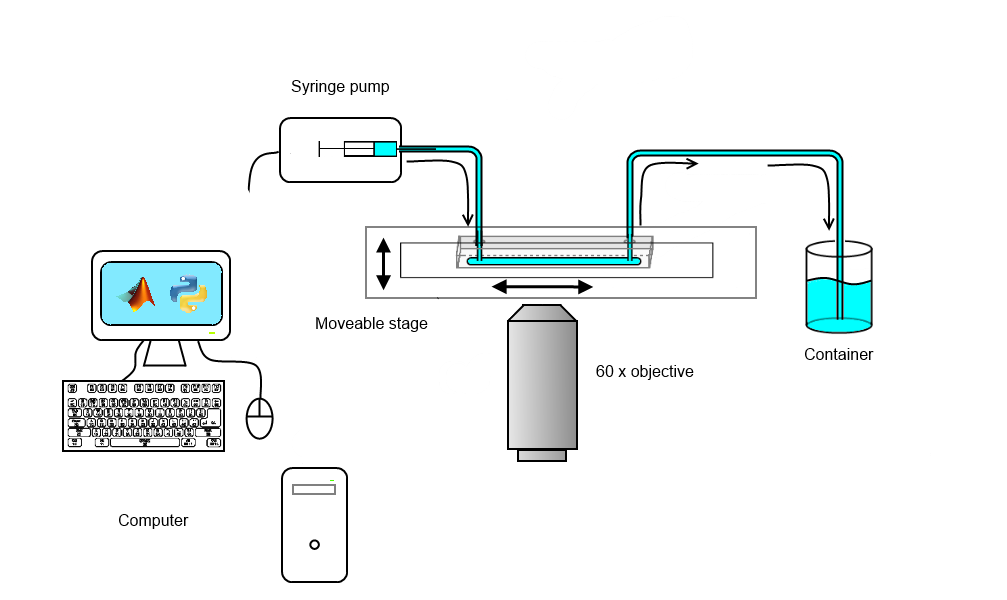
\includegraphics[width=0.8\textwidth]{figures/method/setupsketch.png}
\caption{Sketch of the set up. The computer controlled stage moves over the microscope. The pump reverses when the tracked particle gets close to the inlets of the channel.}\label{fig:setupsketch}
\end{figure}

% Have both this zoomed out and the zoomed in view I think
\begin{figure}[H]
\centering
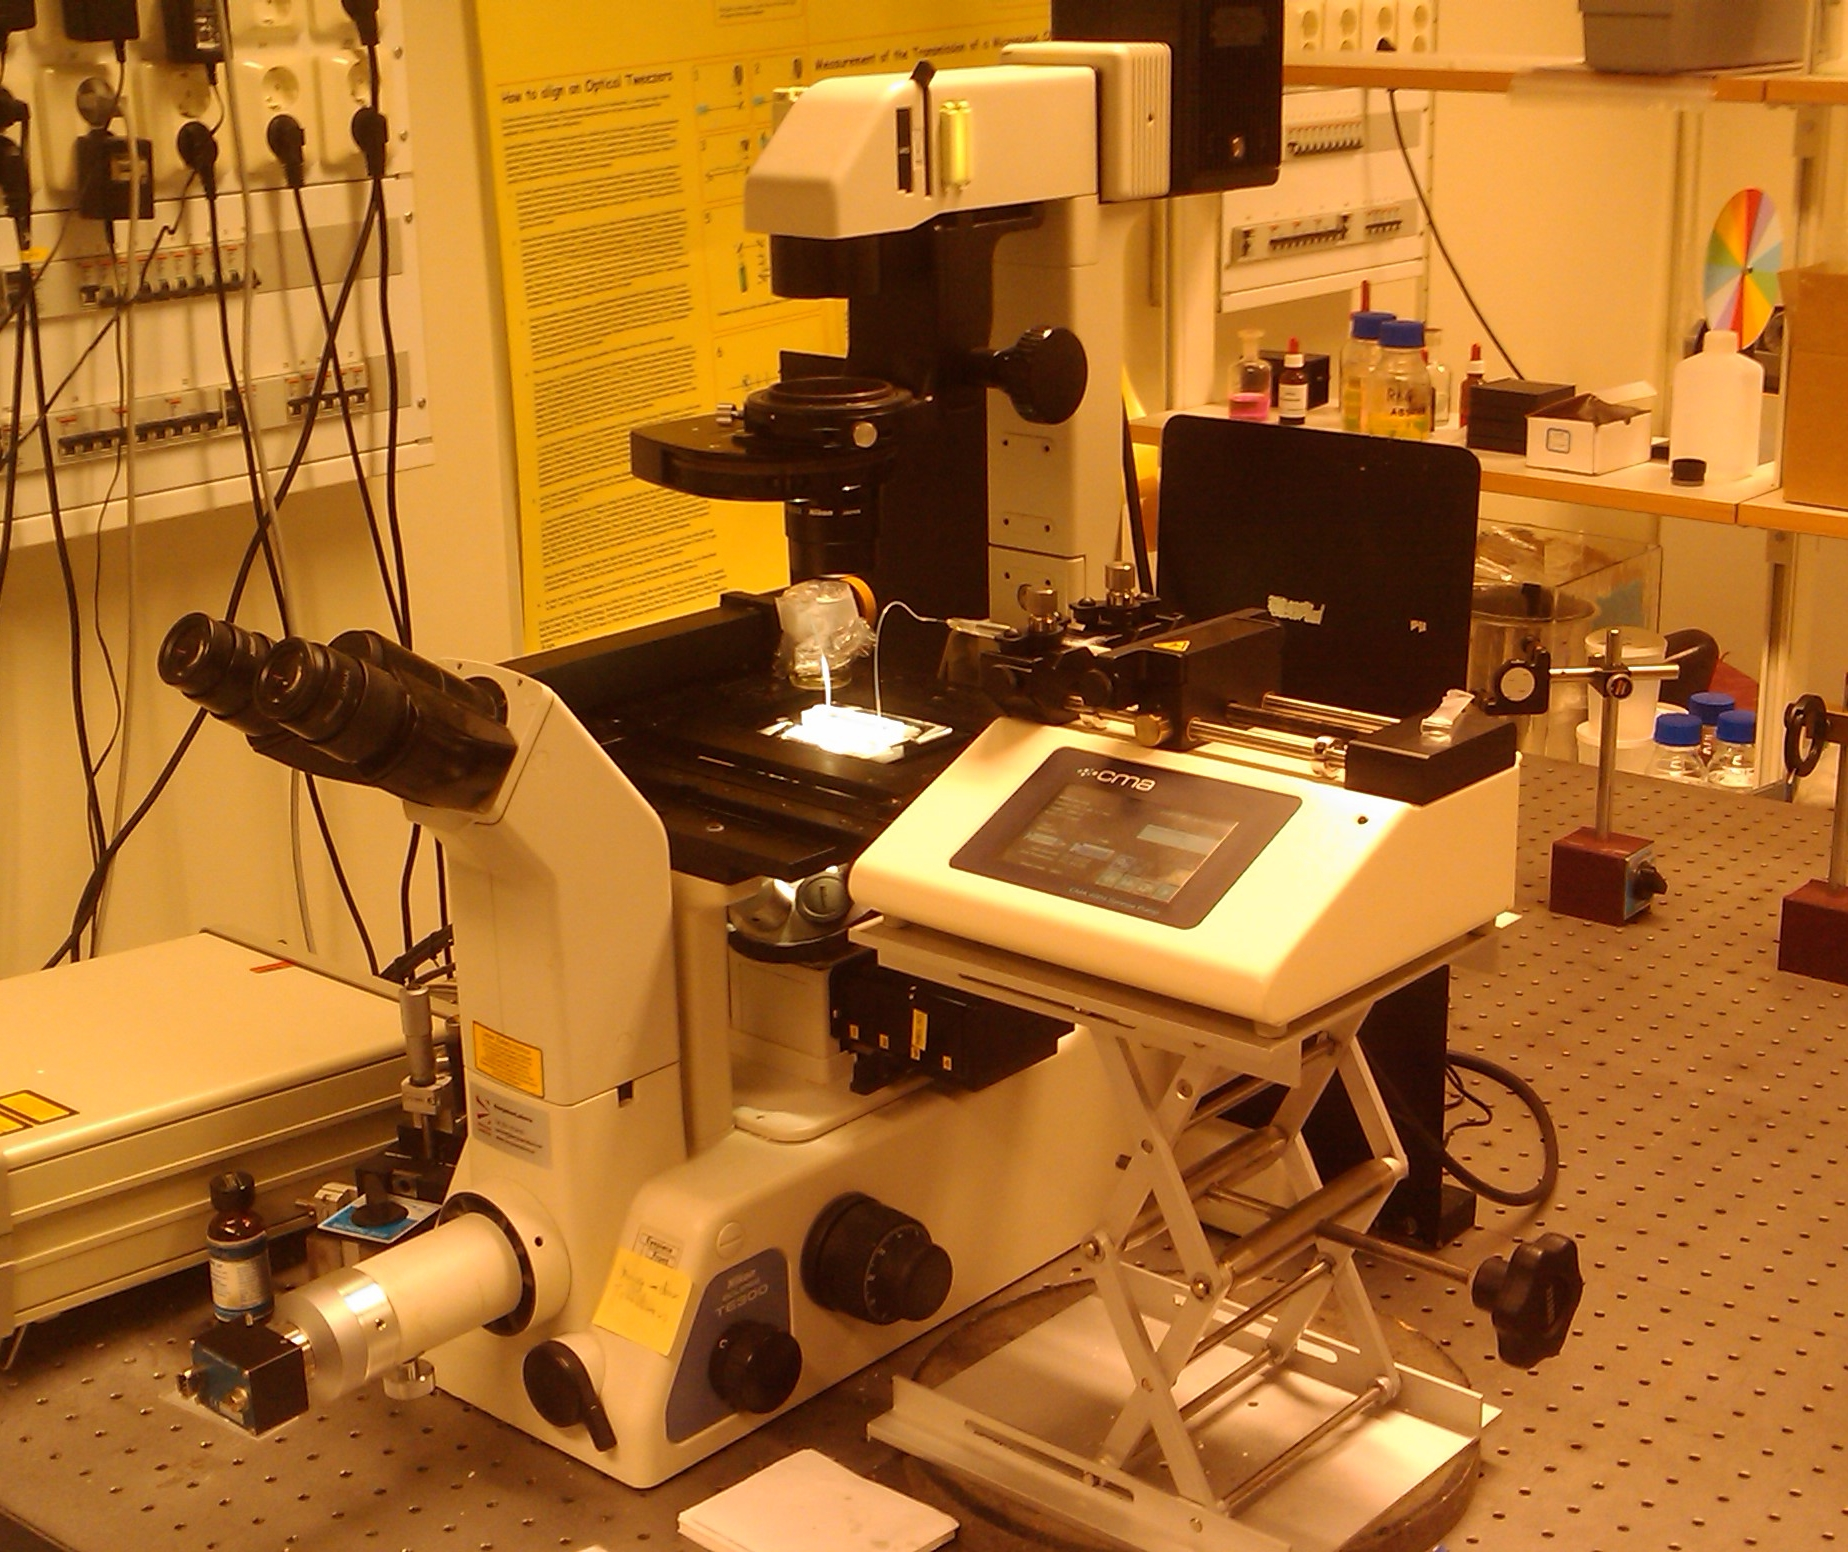
\includegraphics[width=0.8\textwidth]{figures/method/ExperimentalOverview.jpg}
\caption{Overview of the set up. The microscope to the left and the syringe pump to the right. In the center is the channel and the outlet container is seen behind it. The CCD camera is mounted on the left side of the microscope and cannot be seen in this picture.}\label{fig:setuppicture}
\end{figure}


The microfluidic channel is \unit[40]{mm} long, \unit[2.5]{mm} wide and approximately \unit[150]{$\mu$m} deep. The channel is made from Polydimethylsiloxane (PDMS) and plasma bonded to a microscope slide. A more detailed description of the process can be found from the Center for Computer Integrated Systems for Microscopy and Manipulation~\cite{PDMS}. This material and procedure is chosen so that a channel that gets filled with dirt or breaks can cheaply and easily be replaced. PDMS is also non-reactive and highly transparent. A sketch of the channel can be seen in figure \ref{fig:channelsketch}, and a photograph of an actual channel in figure \ref{fig:channelpicture}. 

\begin{figure}[H]
\centering
\begin{subfigure}[b]{0.45\textwidth}
\includegraphics[width=0.9\textwidth]{figures/method/channelDetail.pdf}
\caption{Sketch of the channel}\label{fig:channelsketch}
\end{subfigure}
\begin{subfigure}[b]{0.45\textwidth}
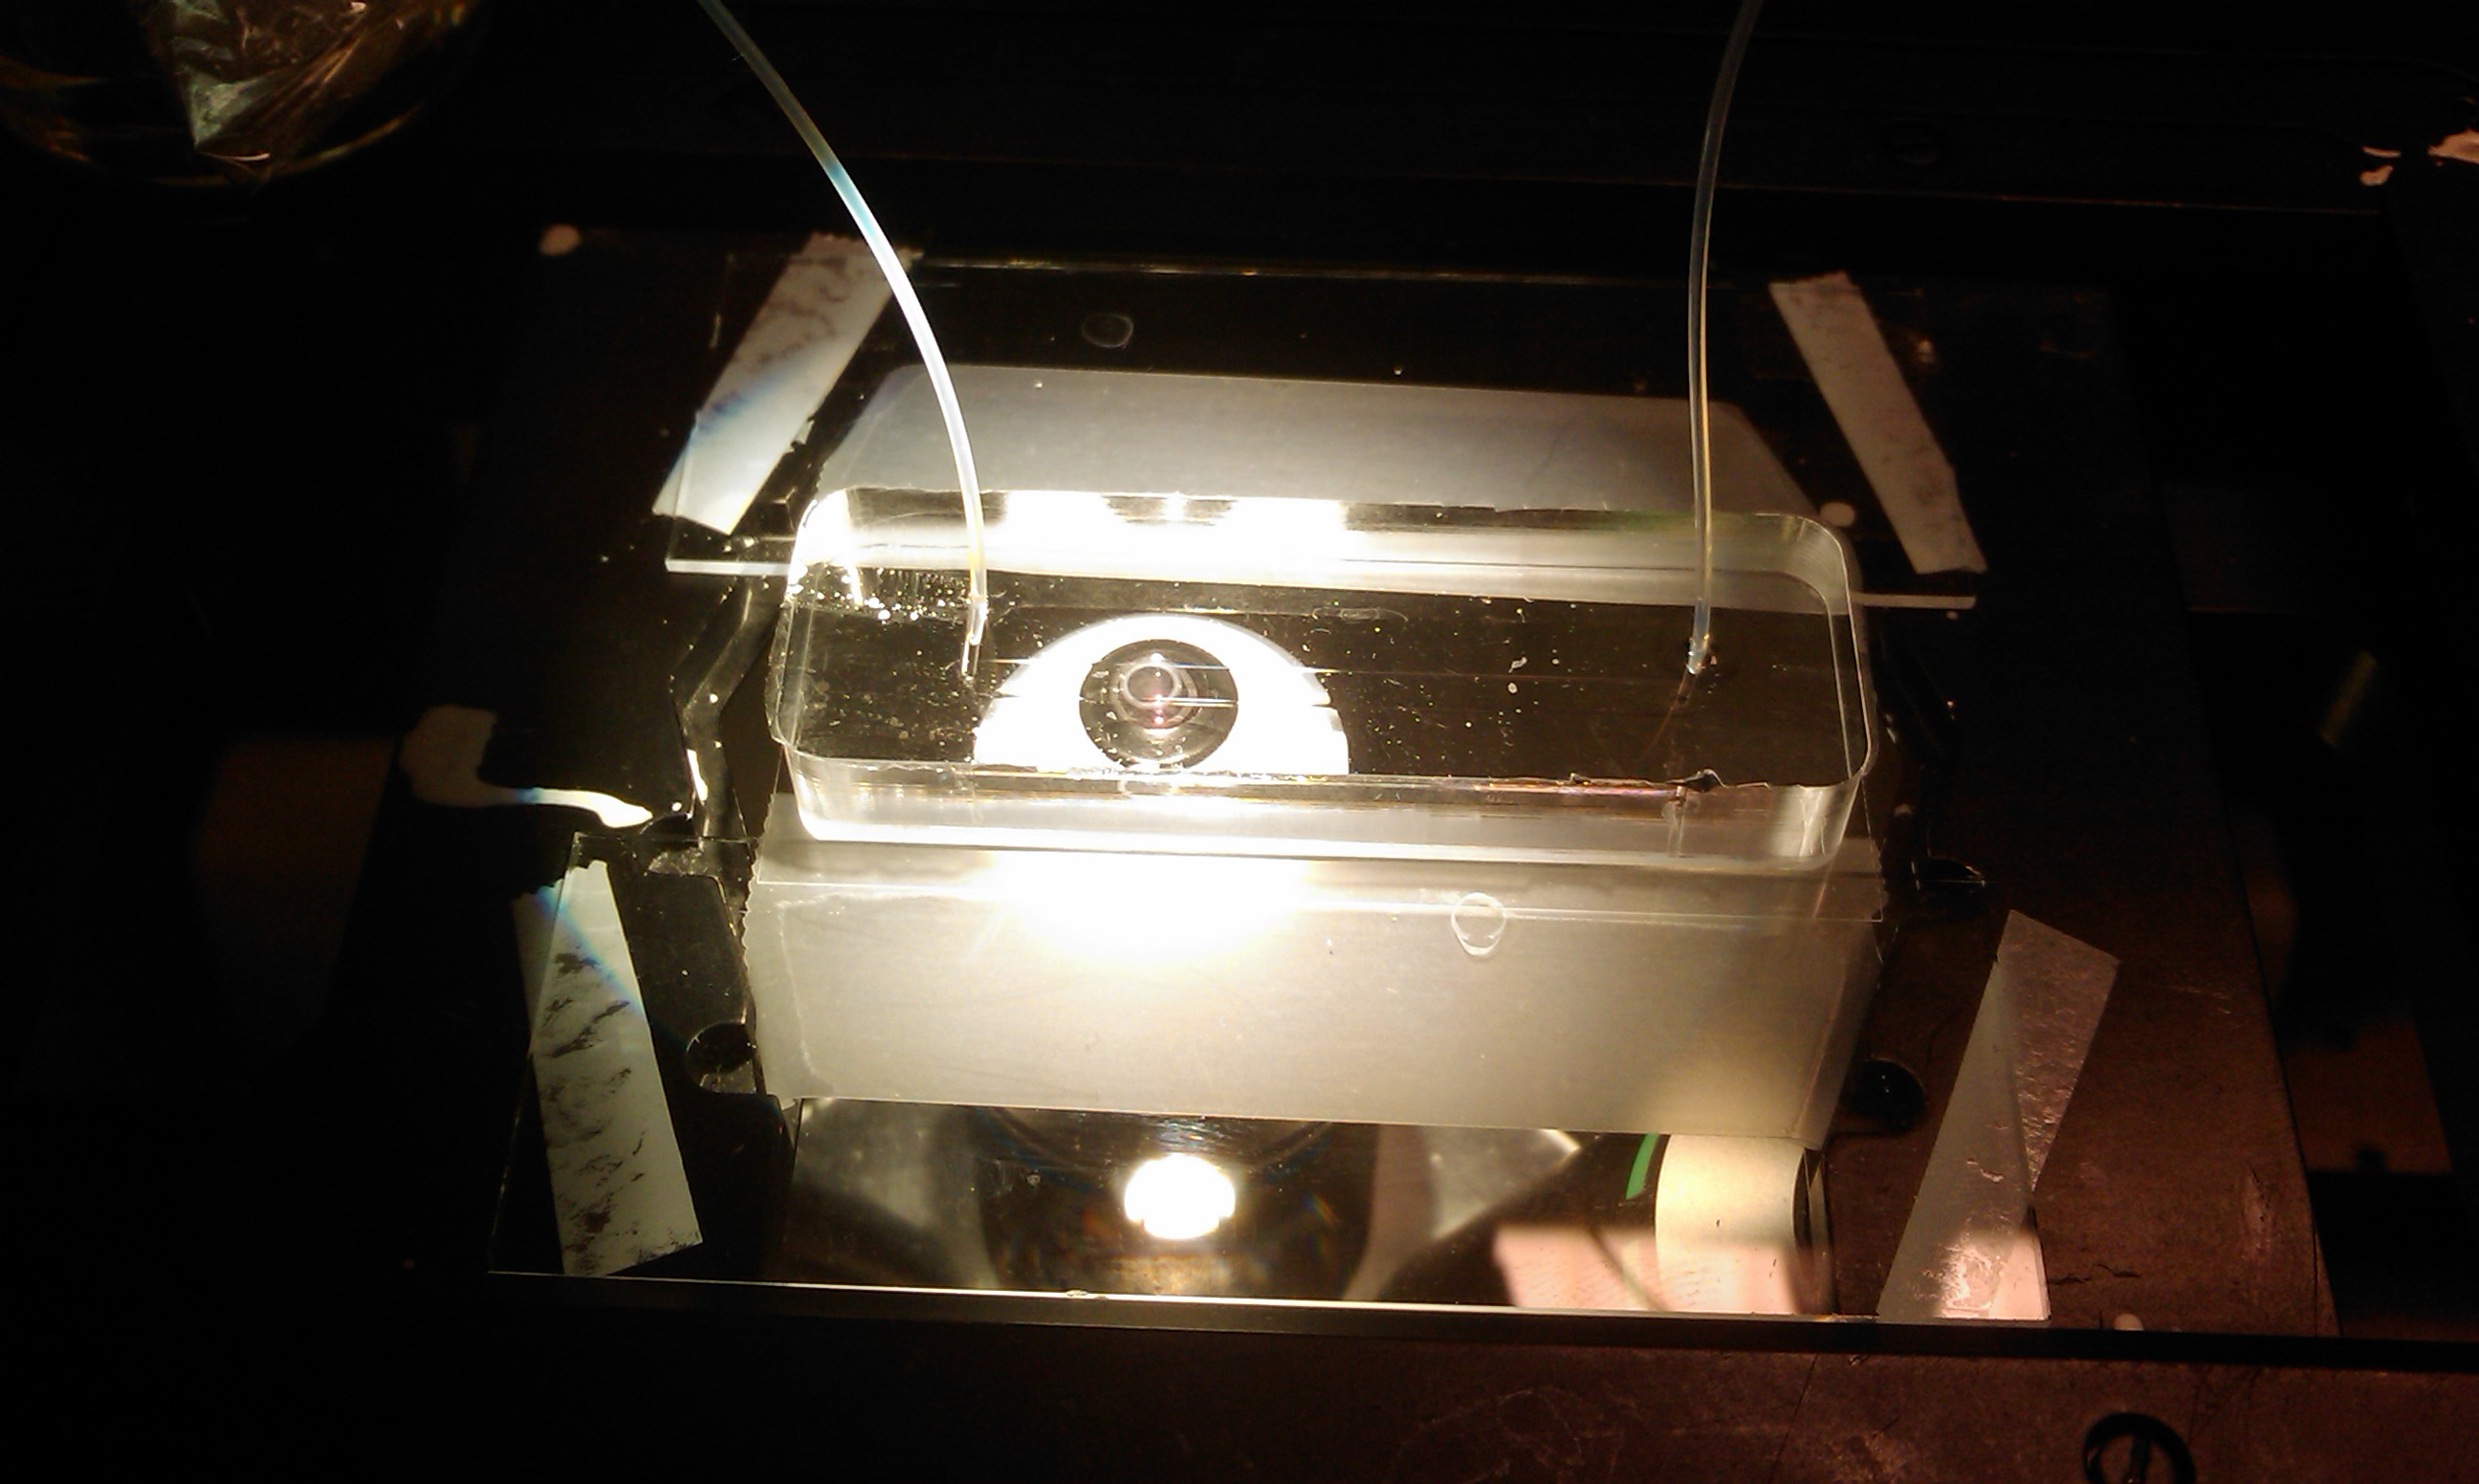
\includegraphics[width=0.9\textwidth]{figures/method/ChannelZoomed.jpg}
\caption{Picture of the channel}\label{fig:channelpicture}
\end{subfigure}
\caption{A sketch of the channel as well as a picture of the channel as it is set up during a measurement. The channel is only \unit[150]{$\mu$m} deep, but the PDMS surrounding it is around 15 mm to try and prevent the channel from expanding and contracting too much.}
\label{fig:channel}
\end{figure}

% rewrite
In order to find the maximum flow speed of the channel we need to know the flow profile. Using the software employed by Johansson \cite{AntonThesis} we obtain the flow profile that can be seen in figure \ref{fig:flowprofile}. Integrating 
the flow profile over the entire surface will give us an effective flow area, essentially how large the channel 'actually' is. 
Using the flow profile from figure \ref{fig:flowprofile} we find that the effective flow area is $\unit[0.14]{mm^2}$. With a pump rate of \unit[7.5]{$\mu$l/minute} we get a maximum velocity of \unit[0.90]{mm/s} for the liquid.

% PIcture of the channel meassurements here 


% Picture of channel flow profile
\begin{figure}[H]
\begin{center}
\includegraphics[width=0.7\textwidth]{figures/method/flowprofile.pdf}
\end{center}
\caption{The theoretical estimation of the flow profile. Image generated with software from Johansson \cite{AntonThesis}, used with permission.}
\label{fig:flowprofile}
\end{figure}

\noindent We need to confirm that the flow is Stokes' flow and thus have no inertial effects. We can calculate the maximum Reynolds number using eq \ref{eq:reynolds}, the \unit[3]{$\mu$m} length rods, and our maximum flow speed.

\begin{equation}
\operatorname{Re} = \frac{U L \rho}{\mu} 
\leq \frac{9.0\cdot 10^{-4} \cdot 3 \cdot 10^{-3} 2.5 }{24 \cdot 10^{-3}} 
\approx	 	2.78  \cdot 10^{-6} \ll 1.
\end{equation}

\noindent This should satisfy the conditions of validity for the Jeffery equations. 

To track the particles the channel is put in a moveable stage on a confocal microscope. The entire setup can be seen in figure \ref{fig:setuppicture}



\subsection{List of equipment}
 The equipment used during the experiment is as follows
\begin{itemize}
\item Leica DFC350 FX digital camera 
\item Nikon Eclipse TE 300 microscope
\item Nikon 60x water immersion objective
\item Märzhäuser Wetzlar 'LStep-eco' step engine
\item CMA 4004 syringe pump
\item Ytterbium fiber laser  % What laser?
\end{itemize}

%
%\subsection{Density matching}
%\begin{equation}
%\rho_{a} = 	\frac {m_{a}}{V_{a}} =
%				\frac{V_{b}\rho_{b} + V_{mix}\rho_{mix}}{V_b + V_{mix}} 
%\end{equation}
%So if we want to find $V_{mix}$ we get
%\begin{equation}
%V_{mix} = \frac{ V_{b}(\rho_{b} - \rho_{a})}{\rho_{a} - \rho_{mix}} 
%\end{equation}
%
	